% H -> WW + charm : analysis status
% LaTeX/Beamer conversion of analysis-overview.md (Marp, 63 slides)
%
% Build:  pdflatex analysis-overview.tex   (twice, for the frame count)
%
\documentclass[aspectratio=169,10pt]{beamer}

\usetheme{default}
\usecolortheme{default}
\setbeamertemplate{navigation symbols}{}
\usefonttheme{professionalfonts}

\usepackage[T1]{fontenc}
\usepackage[utf8]{inputenc}
\usepackage{lmodern}
\usepackage{graphicx}
\usepackage{booktabs}
\usepackage{array}
\usepackage{amsmath}
\usepackage{amssymb}
\usepackage{xcolor}
\usepackage{tcolorbox}
\usepackage{hyperref}
\usepackage{ragged2e}

%% ---- palette, matching the Marp theme -------------------------------------
\definecolor{deckblue}{HTML}{1F4E79}
\definecolor{deckgold}{HTML}{B8862B}
\definecolor{deckred}{HTML}{A01C1C}
\definecolor{keygreen}{HTML}{2F6B3C}
\definecolor{keybg}{HTML}{EDF4ED}
\definecolor{warnorange}{HTML}{B5651D}
\definecolor{warnbg}{HTML}{FBF2E8}
\definecolor{codebg}{HTML}{EBEEF1}
\definecolor{rowgrey}{HTML}{F2F4F6}

\setbeamercolor{frametitle}{fg=deckblue}
\setbeamercolor{title}{fg=deckblue}
\setbeamercolor{structure}{fg=deckblue}
\setbeamerfont{frametitle}{series=\bfseries,size=\large}

%% frame title with the gold rule underneath, as in the Marp theme
\setbeamertemplate{frametitle}{%
  \vspace{0.35em}%
  \usebeamerfont{frametitle}\usebeamercolor[fg]{frametitle}\insertframetitle%
  \vspace{0.15em}\par%
  {\color{deckgold}\rule{\textwidth}{1.2pt}}%
  \vspace{-0.2em}%
}

\setbeamertemplate{footline}{%
  \hfill{\color{gray}\scriptsize\insertframenumber}\hspace{1em}\vspace{0.6em}%
}

%% ---- helpers --------------------------------------------------------------
\newcommand{\code}[1]{{\ttfamily\small\colorbox{codebg}{#1}}}
\newcommand{\hl}[1]{\textcolor{deckred}{\textbf{#1}}}

% key / warn callout boxes (the <div class="key"> and "warn" of the Marp deck)
\newtcolorbox{keybox}{
  colback=keybg, colframe=keygreen, boxrule=0pt, leftrule=3pt,
  arc=0pt, outer arc=0pt, boxsep=2pt, left=6pt, right=6pt, top=4pt, bottom=4pt,
  before skip=4pt, after skip=4pt
}
\newtcolorbox{warnbox}{
  colback=warnbg, colframe=warnorange, boxrule=0pt, leftrule=3pt,
  arc=0pt, outer arc=0pt, boxsep=2pt, left=6pt, right=6pt, top=4pt, bottom=4pt,
  before skip=4pt, after skip=4pt
}

% section divider frame
\newcommand{\sectionframe}[2][]{%
  \begingroup
  \setbeamercolor{background canvas}{bg=deckblue}
  \begin{frame}[plain]
    \vfill
    \begin{center}
      {\Large\bfseries\color{white} #2}\\[0.4em]
      \colorbox{deckgold}{\makebox[0.35\textwidth]{\rule{0pt}{1.2pt}}}
      \ifx\relax#1\relax\else\\[0.6em]{\color{white!80!deckblue}\small #1}\fi
    \end{center}
    \vfill
  \end{frame}
  \endgroup
}

\renewcommand{\arraystretch}{1.25}

\title{H $\rightarrow$ WW + charm}
\subtitle{Analysis status}
\author{Chirayu Gupta \textperiodcentered\ VUB}
\date{August 2026}

\begin{document}

%% ===========================================================================
{\setbeamercolor{background canvas}{bg=deckblue}
\begin{frame}[plain]
  \vfill
  \begin{center}
    {\Huge\bfseries\color{white} H $\rightarrow$ WW + charm}\\[0.5em]
    \colorbox{deckgold}{\makebox[0.4\textwidth]{\rule{0pt}{1.4pt}}}\\[0.8em]
    {\Large\color{white} Analysis status}\\[1.4em]
    {\color{white!85!deckblue} Chirayu Gupta \textperiodcentered\ VUB \textperiodcentered\ August 2026}\\[1.6em]
    {\color{white}\textbf{2022postEE \textperiodcentered\ 26.7 fb$^{-1}$ \textperiodcentered\ expected UL 1034}}
  \end{center}
  \vfill
\end{frame}}

%% ---------------------------------------------------------------------------
\begin{frame}{Sections}
\vspace{0.5em}
\begin{center}
\begin{tabular}{cl}
\toprule
\textsection & topic \\
\midrule
1 & Analysis and selection \\
2 & MVA-defined regions \\
3 & c-tagging --- 2D working points and scale factors \\
4 & Negative-weight reweighting \\
5 & W+jets jet-binned samples \\
6 & Systematics and impacts \\
7 & Status and outlook \\
\bottomrule
\end{tabular}
\end{center}
\end{frame}

%% ===========================================================================
\sectionframe{1 \textperiodcentered\ Analysis and selection}

\begin{frame}{Why H+c}
The Higgs coupling to \textbf{charm} is the least constrained of the accessible
Yukawas. Associated production \textbf{H + c} probes it directly, without relying
on the H$\rightarrow$c$\bar{\text{c}}$ decay.
\vspace{0.4em}
\begin{center}
\begin{tabular}{ll}
\toprule
\textbf{production} & pp $\rightarrow$ H + c (+X) \\
decay & H $\rightarrow$ WW* $\rightarrow$ 2$\ell$2$\nu$ \\
final state & \textbf{opposite-sign e$\mu$} + MET + $\geq$1 c-tagged jet \\
dataset & 2022postEE, \textbf{26.7 fb$^{-1}$}, ReReco \code{22Sep2023} \\
\bottomrule
\end{tabular}
\end{center}
\vspace{0.3em}
\begin{keybox}
The e$\mu$ requirement removes Z$\rightarrow$ee/$\mu\mu$ by construction, so the
irreducible background is \textbf{real t$\bar{\text{t}}$} rather than Drell-Yan.
\end{keybox}
\vspace{0.2em}
{\small Reference: \textbf{AN-23-102}, the full Run 2 analysis at 138 fb$^{-1}$.}
\end{frame}

\begin{frame}{Signal and final state}
\textbf{H $\rightarrow$ WW $\rightarrow$ 2$\ell$2$\nu$, produced with a charm quark.}
Final state: \textbf{opposite-sign e$\mu$} + MET + \textbf{$\geq$1 c-tagged jet}
\vspace{0.3em}
\begin{center}
\small
\begin{tabular}{ll}
\toprule
object & selection \\
\midrule
muons & tight ID + tight PF iso, $p_T > 10$, $|\eta| < 2.4$ \\
electrons & wp80iso, $p_T > 10$, $|\eta| < 2.5$, $\Delta R(e,\mu) > 0.4$ \\
$\ell\ell$ pair & OS, $p_T > 20/10$, pair $p_T > 30$, $m_{\ell\ell} > 12$ \\
jets & $p_T > 30$, $|\eta| < 2.4$, tight-lepveto ID, $\Delta R(j,\ell) > 0.4$ \\
c-jets & $p_T > 20$, \textbf{PNet medium} CvL/CvB \\
MET & PuppiMET \\
\bottomrule
\end{tabular}
\end{center}
\vspace{0.3em}
\begin{keybox}
e$\mu$ removes the Z$\rightarrow$ee/$\mu\mu$ peak \textbf{by construction} --- the
irreducible background is \textbf{real t$\bar{\text{t}}$}, not Drell-Yan.
Triggers: MuonEG, SingleMu, SingleEle.
\end{keybox}
\end{frame}

\begin{frame}{Signal region composition}
\vspace{0.5em}
\begin{center}
\begin{tabular}{lrr}
\toprule
process & SR yield & share of SR \\
\midrule
t$\bar{\text{t}}$ & 17,744 & 82.3\% \\
st & 1,543 & 7.2\% \\
vjets & 1,523 & 7.1\% \\
diboson & 609 & 2.8\% \\
higgsbkg & 132 & 0.6\% \\
\textbf{H+c signal} & \textbf{0.26} & \textbf{0.001\%} \\
\midrule
\textbf{total} & \textbf{21,552} & \\
\bottomrule
\end{tabular}
\end{center}
\end{frame}

%% ===========================================================================
\sectionframe{2 \textperiodcentered\ MVA-defined regions}

\begin{frame}{Six classes, one network}
\vspace{0.4em}
\begin{center}
\begin{tabular}{ll}
\toprule
setting & value \\
\midrule
model & \code{SimpleMLP\_MultiClass} (b-hive) \\
classes & \code{hplusc, higgsbkg, tt, st, diboson, vjets} \\
features & \textbf{26}, including the \textbf{11 c-tag one-hot categories} \\
training & 30 epochs, batch 1024, lr 1e-3, loss weighting on \\
split & 80/20, deterministic by NanoAOD \code{event} id \\
\bottomrule
\end{tabular}
\end{center}
\vspace{0.4em}
\begin{keybox}
The 11 one-hot categories mean the network sees the \textbf{full 2D CvL/CvB plane}
--- the same information the scale factors are binned in, not a binary pass/fail.
\end{keybox}
\end{frame}

\begin{frame}{argmax defines the regions}
\textbf{The winning class picks the channel; the winning score is the discriminant.}
\vspace{0.4em}
\begin{center}
\begin{tabular}{lrl}
\toprule
region & events & dominant process \\
\midrule
SR\_hplusc & 21,552 & \textbf{tt 82.3\%} \\
CR\_higgsbkg & 9,220 & tt 86.4\% \\
CR\_tt & 44,199 & \textbf{tt 94.1\%} \\
CR\_st & 20,135 & tt 87.6\% \\
CR\_diboson & 6,585 & tt 72.4\% \\
CR\_vjets & 9,214 & \textbf{vjets 43.2\%} \\
\bottomrule
\end{tabular}
\end{center}
\vspace{0.4em}
Regions are \textbf{orthogonal by construction} --- no cut optimisation to tune or
defend, and every event is used somewhere.
\end{frame}

\begin{frame}{Four of five CRs are tt-dominated --- by design}
The SR is itself \textbf{82\% tt}: in an e$\mu$ final state t$\bar{\text{t}}$ is
dominant everywhere, so a tt-rich CR is expected, not a failure.
\begin{keybox}
\textbf{CR\_tt: 94.1\% purity over 44k events.} It pins the free-floating
\code{rate\_tt}, which covers 82\% of the SR --- the single most valuable
constraint in the fit.
\end{keybox}
\textbf{CR\_vjets holds 59.6\% of all V+jets} in the fit. Without it there is no
V+jets constraint from anywhere.
\begin{warnbox}
Collapsing the CRs to single bins was \textbf{measured}: +33 units for three CRs,
$\sim$+50 for all five. The shapes carry real constraint, so all six channels keep
10 bins.
\end{warnbox}
\end{frame}

\begin{frame}{Templates entering the fit}
\begin{center}
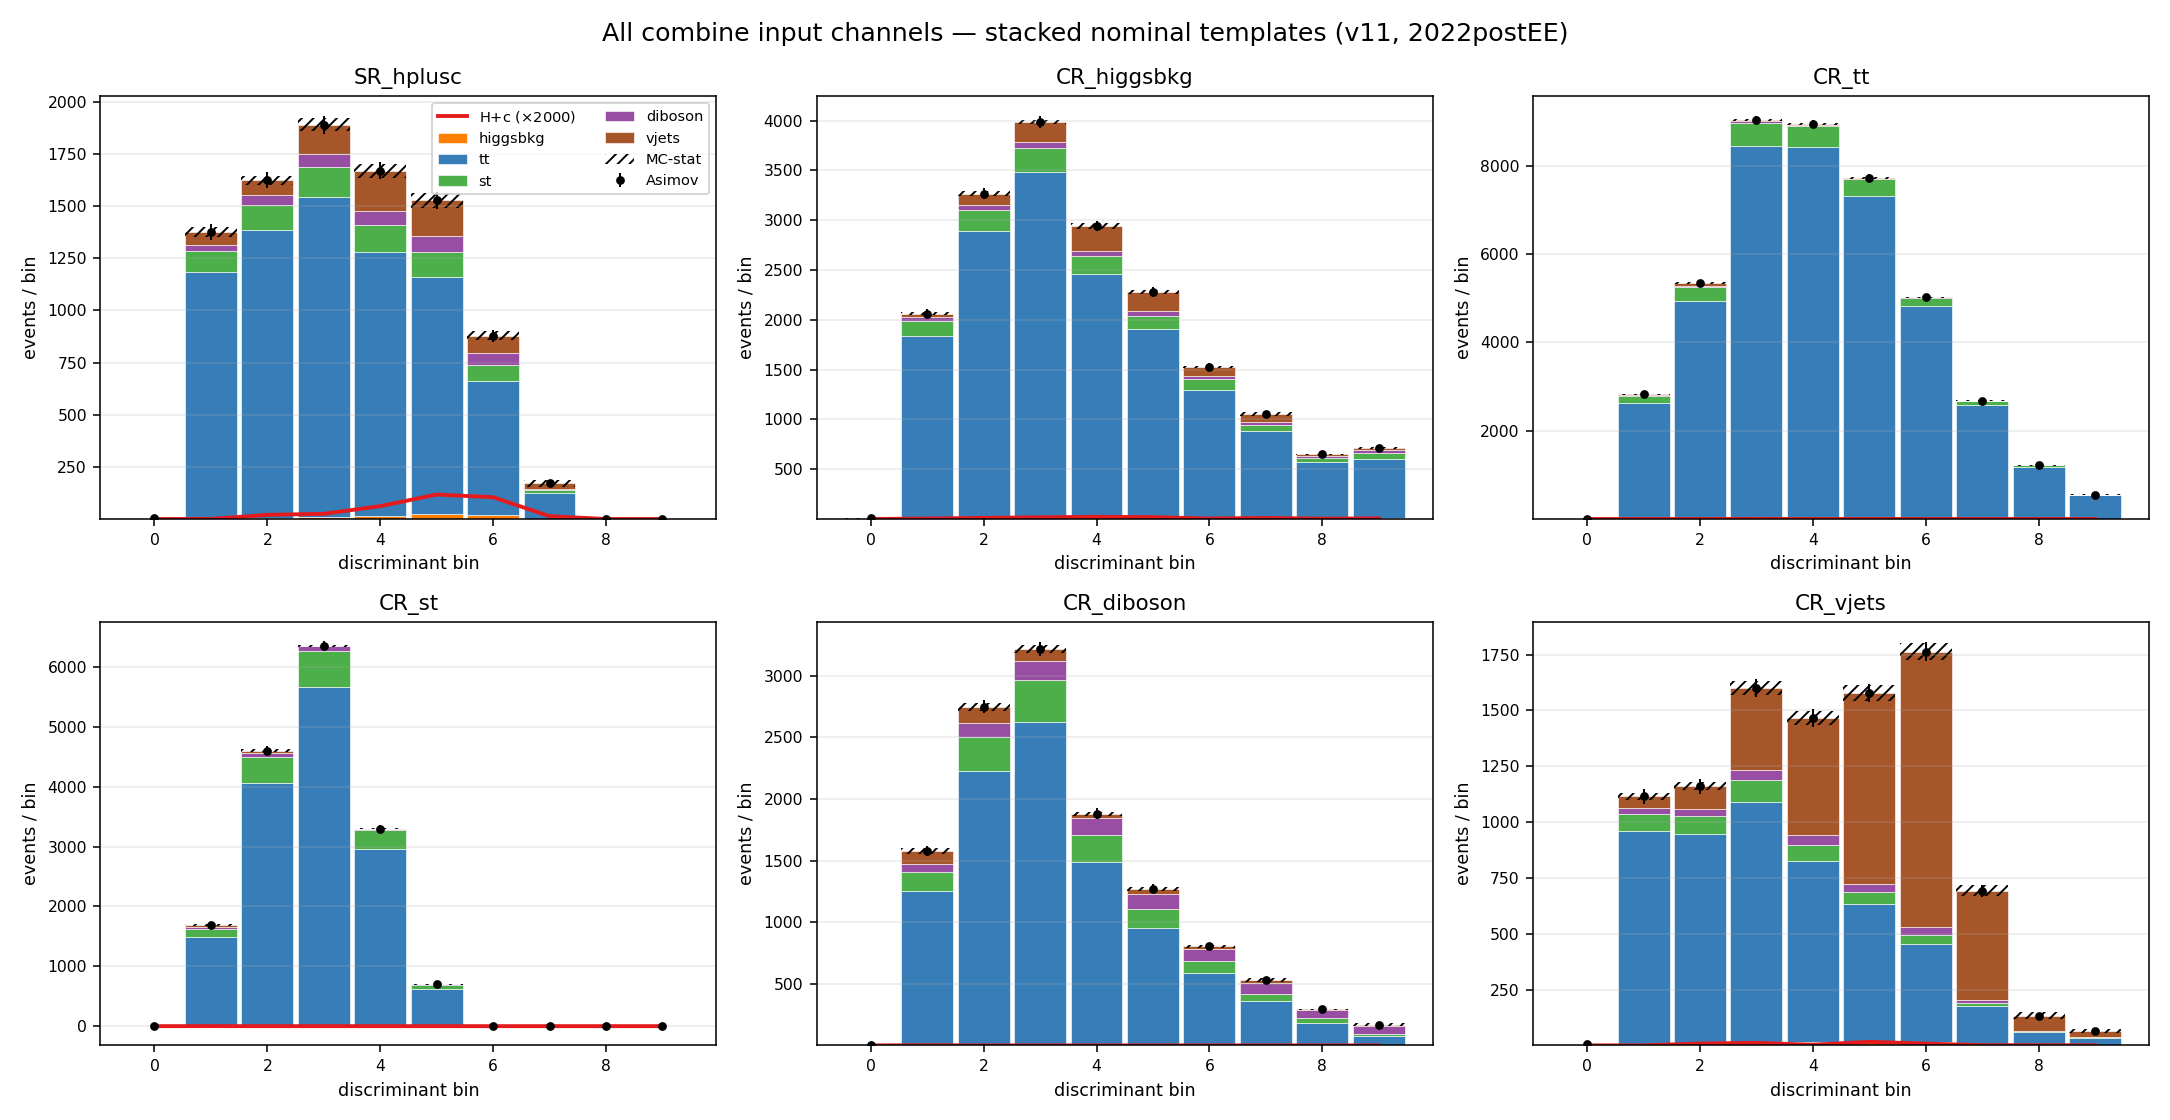
\includegraphics[width=0.82\textwidth]{img/B1_all_channels_stacked.png}
\end{center}
\vspace{0.2em}
{\small 6 channels $\times$ 6 processes $\times$ 10 bins. \textbf{CR\_vjets}
(bottom right) is the only region where V+jets (orange) is visible --- it carries
59.6\% of all V+jets in the fit.}
\end{frame}

%% ===========================================================================
\sectionframe[2D working points and scale factors]{3 \textperiodcentered\ c-tagging}

\begin{frame}{From working points to a plane}
PNet gives \textbf{two} discriminants per jet: \textbf{CvL} (charm vs light) and
\textbf{CvB} (charm vs bottom). A single working-point cut throws most of that away.
The calibration instead partitions the \textbf{whole plane} into \textbf{11
categories} \code{L0, C0--C4, B0--B4} --- including the untagged \code{L0} bin.
\vspace{0.3em}
\begin{center}
\small
\begin{tabular}{ll}
\toprule
property & value \\
\midrule
axes & CvL, CvB --- \textbf{verified sufficient}, no third variable needed \\
categories & 11: \code{L0}, \code{C0}--\code{C4}, \code{B0}--\code{B4} \\
index & computed from CvL/CvB \textbf{already stored per jet} \\
applied & natively in the processor (\code{CTag2DCorrector}) \\
\bottomrule
\end{tabular}
\end{center}
\vspace{0.3em}
\begin{keybox}
Because the scheme spans the \textbf{full plane including \code{L0}}, the SF
machinery works even for a selection with no working point at all.
\end{keybox}
\end{frame}

\begin{frame}{Only 7 of 11 categories are populated}
{\small Occupancy of the five largest (\code{C4} and \code{B0} are populated but sparse):}
\vspace{0.3em}
\begin{center}
\small
\begin{tabular}{lrrrr}
\toprule
category & jets & c (\%) & b (\%) & light (\%) \\
\midrule
\code{L0} & 130,694 & 13.5 & 4.7 & \textbf{81.8} \\
\code{C0} & 188,702 & 28.2 & 6.2 & 65.7 \\
\code{C1} & 170,043 & 58.0 & 7.9 & 34.1 \\
\code{C2} & 17,823 & 58.6 & 33.4 & 8.0 \\
\code{C3} & 1,082 & 30.6 & \textbf{57.9} & 11.5 \\
\bottomrule
\end{tabular}
\end{center}
\vspace{0.3em}
The scheme targets a broader phase space than ours --- the b-rich \code{B1}--\code{B4}
categories are empty after the e$\mu$ + c-jet selection.
\begin{keybox}
Category index is computed from CvL/CvB already stored per jet --- \textbf{no
NanoAOD reprocessing was ever needed}.
\end{keybox}
\end{frame}

\begin{frame}{The scale factor matrix}
\begin{center}
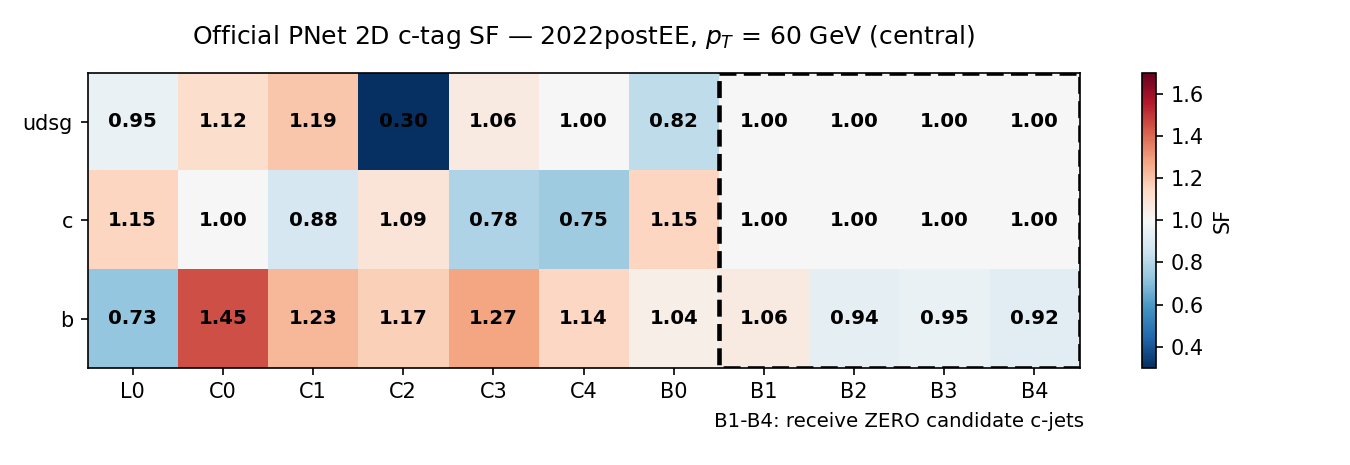
\includegraphics[width=0.78\textwidth]{img/C1_sf_matrix.png}
\end{center}
\end{frame}

\begin{frame}{The uncertainty band is the nuisance}
\begin{center}
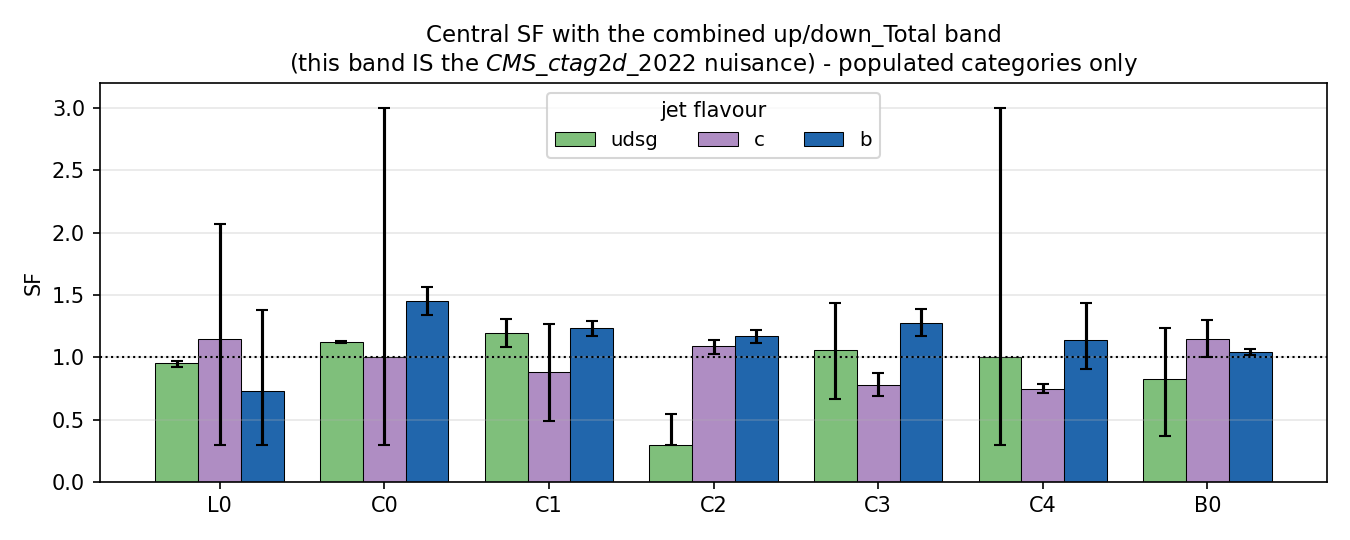
\includegraphics[width=0.76\textwidth]{img/C2_sf_band.png}
\end{center}
\end{frame}

\begin{frame}{What the calibration costs}
\vspace{0.6em}
\begin{center}
\begin{tabular}{lr}
\toprule
configuration & limit \\
\midrule
no SF & 1150 \\
\textbf{+ \code{CMS\_ctag2d\_2022}} & \textbf{1164} \\
\bottomrule
\end{tabular}
\end{center}
\vspace{0.5em}
\begin{keybox}
Applying the calibration \textbf{worsens} the limit by 14 units --- as it must.
A scale factor adds a nuisance. The point is correctness.
\end{keybox}
\begin{warnbox}
Currently \textbf{one nuisance} covering the whole plane. Decorrelation is pending.
\end{warnbox}
\end{frame}

%% ===========================================================================
\sectionframe[full detail: \texttt{negrw-deck.pdf} (57 slides)]{4 \textperiodcentered\ Negative-weight reweighting}

\begin{frame}{The estimator is a cancellation}
aMC@NLO events carry \textbf{signed} weights. The yield estimator
\begin{equation*}
\hat{N}_B = \sum_{i \in B} w_i, \qquad w_i = \pm|w_i|
\end{equation*}
is a \textbf{difference of two large numbers}.
\begin{itemize}
  \item the \textbf{expectation} is correct --- the yield is unbiased
  \item the \textbf{variance} is not: it scales with $\sum w_i^2 = \sum|w_i|^2$, the
        \emph{unsigned} statistics, while the mean is the much smaller signed sum
  \item effective statistics collapse: $N_{eff} = (\sum w)^2/\sum w^2 \ll N$
\end{itemize}
\begin{warnbox}
\textbf{16.4\%} of our V+jets events carried a negative weight. In a sparse bin the
positives and negatives can cancel \textbf{completely} --- leaving zero content with
a large finite error.
\end{warnbox}
\end{frame}

\begin{frame}{V+jets was starved exactly under the signal}
\begin{center}
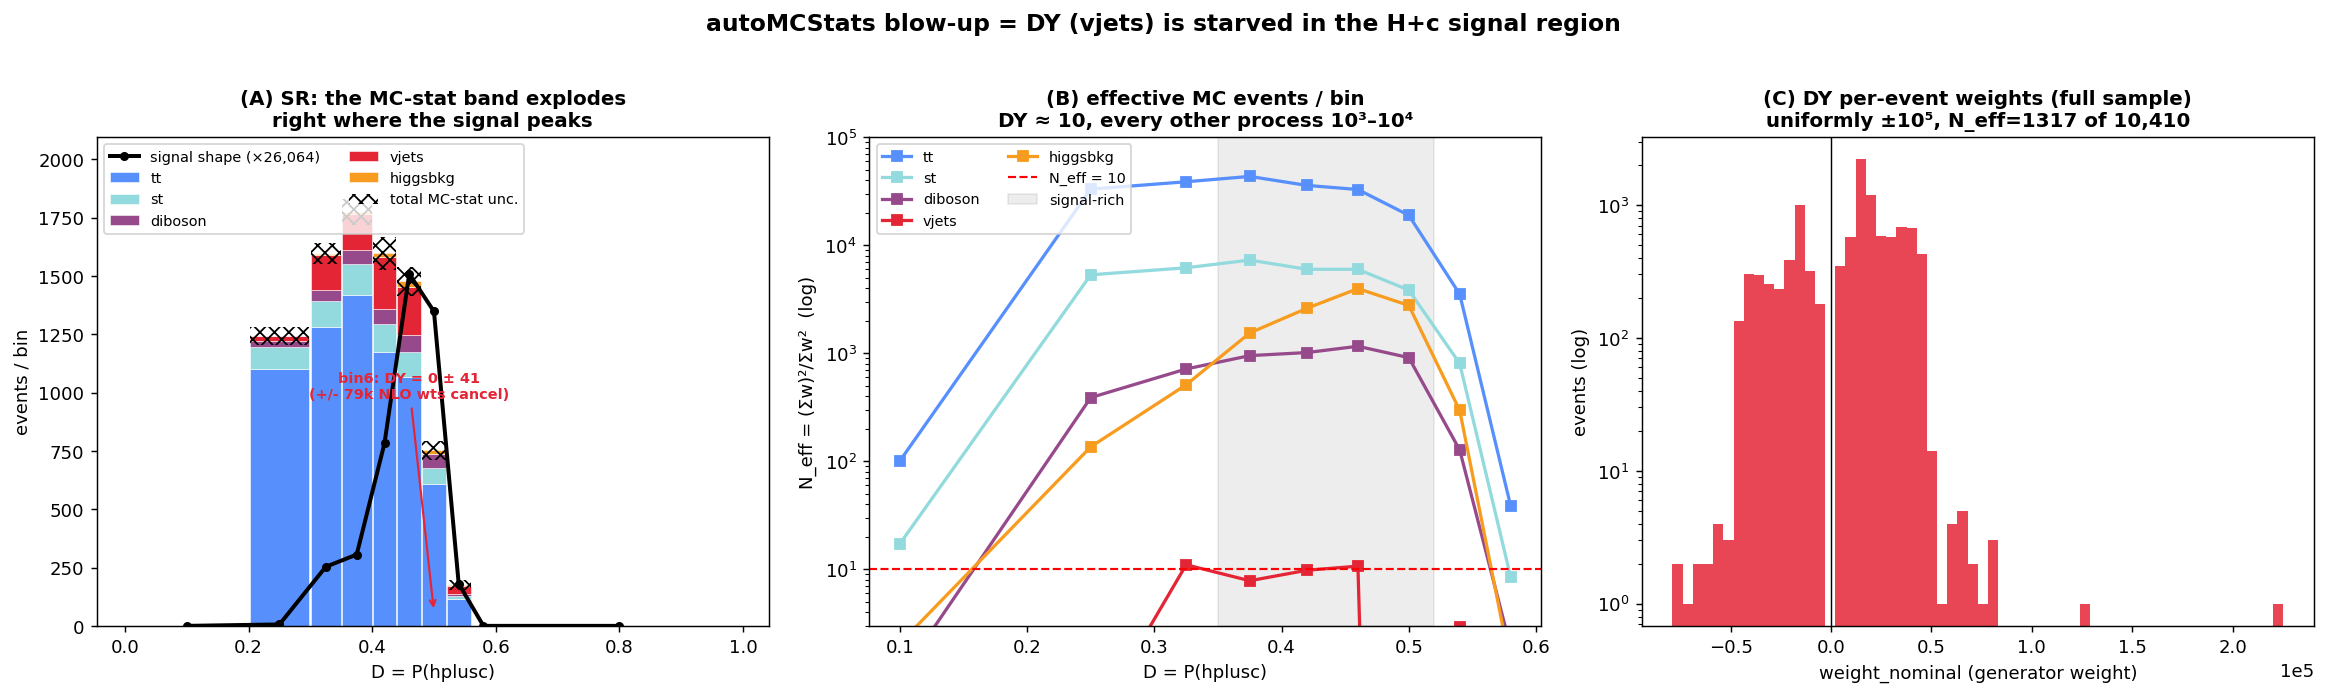
\includegraphics[width=0.94\textwidth]{img/automcstats_issue.png}
\end{center}
\vspace{0.2em}
{\small \textbf{(A)} the MC-stat band explodes where the signal peaks --- one bin was
DY $= 0 \pm 41$ from $\pm$79k weights cancelling \textperiodcentered\ \textbf{(B)}
$N_{eff}$ per bin: V+jets $\approx$10, every other process $10^3$--$10^4$
\textperiodcentered\ \textbf{(C)} DY per-event weights, uniformly $\pm10^5$}
\end{frame}

\begin{frame}{The method --- an algebraic identity}
Write the signed generator density as a difference of two positive densities:
\begin{equation*}
\text{PDF}(\vec{x}) = a\,\text{PDF}_+ - b\,\text{PDF}_-, \qquad a-b=1
\end{equation*}
With $P_+(\vec{x}) = a\text{PDF}_+ / (a\text{PDF}_+ + b\text{PDF}_-)$:
\begin{equation*}
\text{PDF}(\vec{x}) = \underbrace{(2P_+(\vec{x})-1)}_{g(\vec{x})}\cdot
(a\text{PDF}_+ + b\text{PDF}_-)
\end{equation*}
The right factor is the \textbf{unsigned} density --- what $\sum|w|$ samples.
\begin{keybox}
So $\sum|w|\,g$ and $\sum w$ estimate \textbf{the same distribution}.
Yield-preserving by construction, not an approximation.
\end{keybox}
{\small Exact for the \emph{true} $P_+$. We use $\hat{P}_+$ from a finite classifier
--- so closure becomes an \textbf{empirical} property that must be measured.}
\end{frame}

\begin{frame}{Training region --- train loose, infer tight}
$g(\vec{x})$ is a \textbf{generator property}; it does not know about the analysis
selection. So we train on a far larger sample than the SR.
\vspace{0.4em}
\begin{center}
\begin{tabular}{ll}
\toprule
 & region \\
\midrule
\textbf{train} & all base cuts + veto of the e$\mu$ SR topology \\
\textbf{infer} & the tight e$\mu$ signal region \\
\bottomrule
\end{tabular}
\end{center}
\vspace{0.4em}
\begin{keybox}
\textbf{Disjoint by construction.} An event that is not ``exactly one e$\mu$ pair''
can never be an SR event --- no event-id bookkeeping needed.
\end{keybox}
{\small Rejected alternatives: inverting MET (kinematically softer $\rightarrow$
extrapolation) and inverting the c-jet requirement (flips into the \emph{opposite}
gen corner).}
\end{frame}

\begin{frame}{Inputs --- 20 generator-level features}
\vspace{0.3em}
\begin{center}
\small
\begin{tabular}{ll}
\toprule
group & variables \\
\midrule
LHE event & \code{lhe\_njets}, \code{lhe\_nb}, \code{lhe\_nc}, \code{lhe\_nuds}, \code{lhe\_nglu}, \code{lhe\_npnlo} \\
LHE kinematics & \code{lhe\_ht}, \code{lhe\_htincoming}, \code{lhe\_vpt}, \code{lhe\_alphas} \\
gen partons & multiplicity, \code{n\_pt20/100/200}, incoming PDG IDs \\
leading partons & \code{genparton1/2\_pt}, \code{genparton1/2\_eta} \\
\bottomrule
\end{tabular}
\end{center}
\vspace{0.4em}
\begin{keybox}
\textbf{All generator-level.} The paper explicitly \textbf{rejects reco-level
variables} --- closure is only guaranteed on quantities the generator itself sampled.
\end{keybox}
The two weight classes separate visibly in nearly every one of these features.
\end{frame}

\begin{frame}{The classifier}
\vspace{0.4em}
\begin{center}
\begin{tabular}{ll}
\toprule
setting & value \\
\midrule
model & \code{HistGradientBoostingClassifier} (scikit-learn) \\
inputs & 20 generator-level (\code{lhe\_*}, \code{genparton\_*}) \\
training events & 9.8M \\
\textbf{ensemble AUC} & \textbf{0.829} \\
\bottomrule
\end{tabular}
\end{center}
\vspace{0.4em}
\begin{keybox}
AUC 0.83 on an \textbf{intrinsically stochastic} target --- the weight sign is not a
deterministic function of the kinematics, so a perfect classifier cannot exist even
in principle. 0.83 means the generator-level features genuinely carry the
information the NLO subtraction encodes.
\end{keybox}
\end{frame}

\begin{frame}{Classifier ROC}
\begin{center}
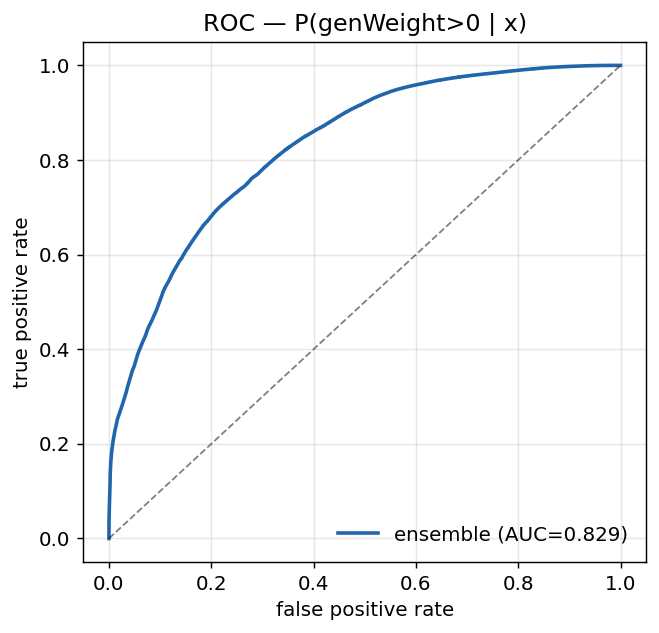
\includegraphics[width=0.50\textwidth]{img/03_roc.png}
\end{center}
\end{frame}

\begin{frame}{The reweight factor and its spread}
\begin{center}
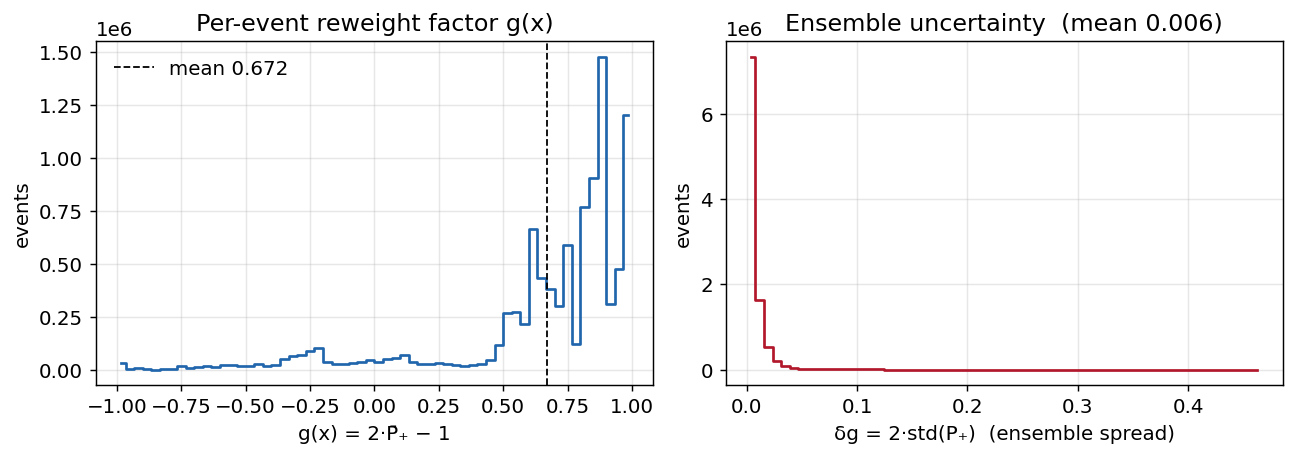
\includegraphics[width=0.58\textwidth]{img/06_g_and_dg.png}
\end{center}
\vspace{0.2em}
{\small $g$ mean \textbf{0.672} $= 2\times0.836-1$, matching the global positive
fraction \textperiodcentered\ range $[-0.991, 0.993]$, inside the physical $[-1,1]$
\textperiodcentered\ $\delta g$ mean \textbf{0.006}, which becomes the
\code{CMS\_negrw\_vjets} nuisance.}
\end{frame}

\begin{frame}{Is $P_+$ calibrated outside the training region?}
\begin{center}
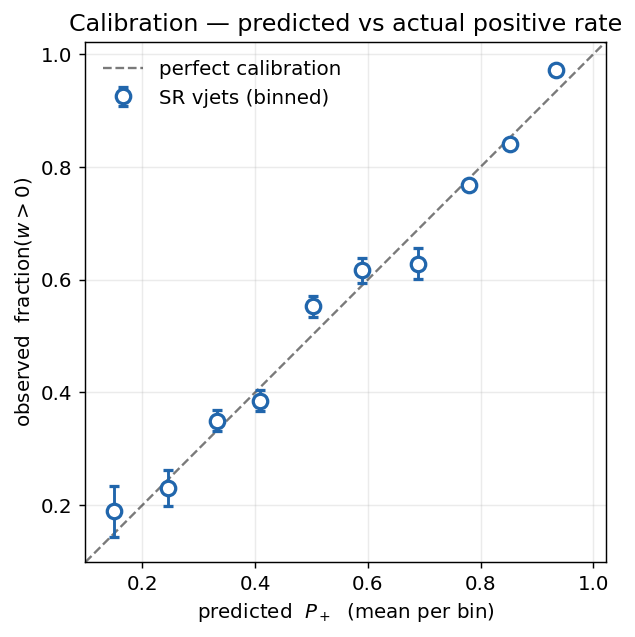
\includegraphics[width=0.40\textwidth]{img/V1_calibration.png}
\end{center}
\vspace{0.2em}
{\small Bin SR events by \textbf{predicted} $P_+$, plot the \textbf{observed}
fraction with $w>0$. Points land on the diagonal across the full range
($P_+ \approx 0.15 \to 0.93$) --- the classifier is calibrated where it is applied,
not only where it was trained.}
\end{frame}

\begin{frame}{Which features carry the information}
\begin{center}
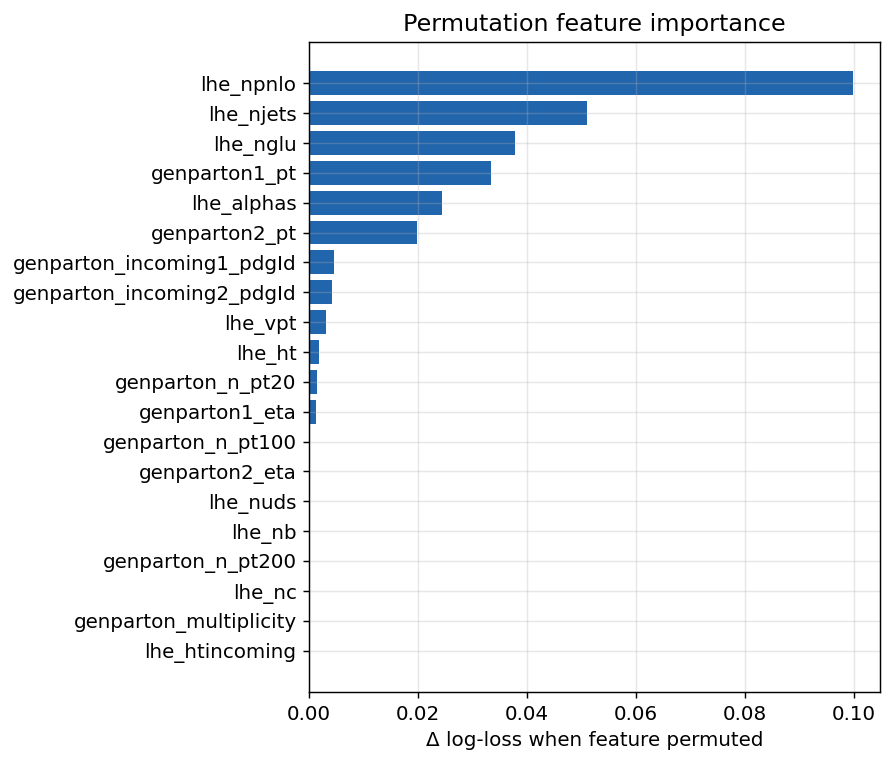
\includegraphics[width=0.50\textwidth]{img/04_feature_importance.png}
\end{center}
\vspace{0.2em}
{\small Permutation importance: the increase in log-loss when a feature is scrambled.}
\end{frame}

\begin{frame}{Closure}
\begin{center}
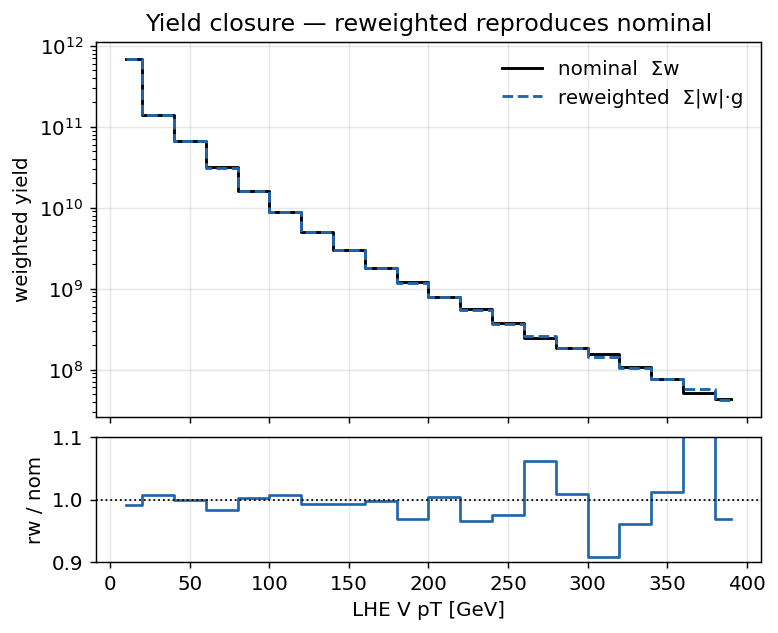
\includegraphics[width=0.54\textwidth]{img/07_closure.png}
\end{center}
\vspace{0.2em}
{\small Training-region closure \textbf{0.994} on 9.8M events --- the reweighting
removes variance and nothing else.}
\end{frame}

\begin{frame}{The gain}
\begin{center}
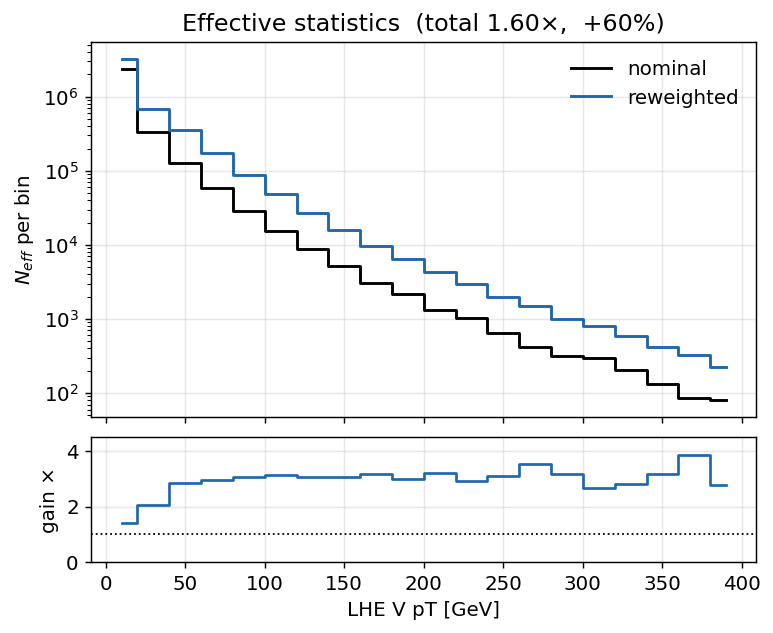
\includegraphics[width=0.56\textwidth]{img/07b_neff_gain.png}
\end{center}
\vspace{0.2em}
{\small Integrated gain \textbf{1.6$\times$}; per-bin ratio $\approx$\textbf{3$\times$}
in the signal-rich bins.}
\end{frame}

\begin{frame}{SR closure and the renormalisation}
{\small The SR is a small, kinematically-biased corner of the training domain, so the
per-event $g$ does not average to the \emph{local} positive fraction.}
\vspace{0.2em}
\begin{center}
\small
\begin{tabular}{lrrr}
\toprule
process & $\sum w$ & $\sum|w|g$ & renorm \\
\midrule
\textbf{DY} (both mass bins) & 1.014e8 & 1.027e8 & \textbf{0.987} \\
\textbf{W$\rightarrow\ell\nu$} & 5.238e7 & 5.876e7 & \textbf{0.891} \\
\bottomrule
\end{tabular}
\end{center}
\vspace{0.2em}
\begin{keybox}
Applied \textbf{per dataset} in the card builder: the reweighted template is scaled
back to the nominal yield, so the \textbf{yield is restored exactly} while the
variance reduction --- from per-bin spread, not the integral --- is untouched.
\end{keybox}
\begin{warnbox}
\textbf{These factors predate the W+jets sample change} --- they are for the old
inclusive \code{WtoLNu\_2Jets}. \textbf{The classifier will be retrained on the
jet-binned 0J/1J/2J samples} and the factors re-derived.
\end{warnbox}
\end{frame}

%% ===========================================================================
\sectionframe{5 \textperiodcentered\ W+jets jet-binned samples}

\begin{frame}{Inclusive $\rightarrow$ jet-binned}
{\small AN-23-102 \textsection2.3 rejects the inclusive NLO sample outright:
\emph{``not used\ldots 5 times smaller than LO and with large fraction of negative
weights.''}}
\vspace{0.2em}
\begin{center}
\small
\begin{tabular}{lrrrr}
\toprule
sample & xsec (pb) & events & files & neg-w \\
\midrule
\code{WtoLNu-2Jets\_0J} & 55,760 & 678M & 3,432 & 10.2\% \\
\code{WtoLNu-2Jets\_1J} & 9,529 & 523M & 2,669 & 25.7\% \\
\code{WtoLNu-2Jets\_2J} & 3,532 & 345M & 2,135 & 34.7\% \\
\midrule
\textbf{sum} & \textbf{68,821} & \textbf{1,546M} & \textbf{8,236} & \\
\emph{old inclusive} & \emph{67,710} & \emph{282M} & \emph{381} & \emph{16.1\%} \\
\bottomrule
\end{tabular}
\end{center}
\vspace{0.2em}
{\small Cross sections from \textbf{XSDB}; sum within \textbf{+1.6\%} of the
inclusive --- normal NLO merging spread, not a double-count. Measured
negative-weight fractions match XSDB to $\sim$1\%.}
\end{frame}

\begin{frame}{Why the gain is not simply 5.5$\times$}
Raw events rise \textbf{5.5$\times$}, but the useful quantity is effective statistics:
\vspace{0.3em}
\begin{center}
\small
\begin{tabular}{lrr}
\toprule
sample & $n_{eff}/N$ & equivalent lumi \\
\midrule
0J & 0.635 & 7.7 /fb \\
1J & 0.237 & 13.0 /fb \\
2J & 0.094 & 9.1 /fb \\
\midrule
\textbf{combined} & & \textbf{29.8 /fb} \\
\emph{inclusive} & \emph{0.460} & \emph{\textbf{1.9 /fb}} \\
\bottomrule
\end{tabular}
\end{center}
\vspace{0.3em}
{\small The inclusive sample spends most of its cross section on \textbf{0-jet}
events, which almost never survive the $\geq$1 c-jet requirement.}
\begin{keybox}
Of the 4,851 surviving SR events, \textbf{2J alone contributes 69\%} --- despite
being the smallest sample. The jet-binned samples are enriched in exactly what the
selection needs.
\end{keybox}
\end{frame}

\begin{frame}{W+jets result: 1160 $\rightarrow$ 1034}
\vspace{0.5em}
\begin{center}
\begin{tabular}{lrr}
\toprule
 & before & after \\
\midrule
\textbf{expected UL} & 1160 & \textbf{1034} \\
V+jets $n_{eff}$ (SR) & 280 & \textbf{1170} \\
V+jets stat.\ error & 5.98\% & \textbf{2.92\%} \\
V+jets rate & 1508 & 1523 \\
\bottomrule
\end{tabular}
\end{center}
\vspace{0.5em}
\begin{keybox}
\textbf{The rate barely moved while the statistical error halved} --- the signature
of a statistics gain, not a normalisation change.
\end{keybox}
\end{frame}

%% ===========================================================================
\sectionframe{6 \textperiodcentered\ The combine card}

\begin{frame}[fragile]{Card structure}
\begin{semiverbatim}\scriptsize
imax 6      # 6 channels: SR_hplusc + 5 argmax CRs
jmax 5      # 6 processes minus one
kmax *      # nuisances counted automatically

shapes * SR_hplusc  v11_hplusc_2dcat.root \\
         SR_hplusc_$PROCESS  SR_hplusc_$PROCESS_$SYSTEMATIC
   ... one line per channel
\end{semiverbatim}
\vspace{0.3em}
\begin{center}
\small
\begin{tabular}{ll}
\toprule
channels & \code{SR\_hplusc}, \code{CR\_higgsbkg}, \code{CR\_tt}, \code{CR\_st}, \code{CR\_diboson}, \code{CR\_vjets} \\
processes & \code{hplusc}, \code{higgsbkg}, \code{tt}, \code{st}, \code{diboson}, \code{vjets} \\
binning & \textbf{10 bins per channel} --- the winning MVA score \\
histograms & 1,626 in the ROOT file (nominal + all up/down) \\
observation & \code{-1} in every channel --- \textbf{Asimov, blind} \\
\bottomrule
\end{tabular}
\end{center}
\end{frame}

\begin{frame}[fragile]{The two special entries}
\textbf{A free-floating tt normalisation:}
\begin{semiverbatim}\small
rate_tt  rateParam  *  tt  1.0  [0,5]
\end{semiverbatim}
{\small One parameter, \textbf{shared across all six channels}, so CR\_tt (94\% pure,
44k events) determines the tt normalisation in the SR. This is why
t$\bar{\text{t}}$ carries no \code{xsec} lnN --- its rate comes from data, following
AN-23-102.}
\vspace{0.4em}
\textbf{Bin-by-bin MC statistics:}
\begin{semiverbatim}\small
SR_hplusc    autoMCStats 10
CR_higgsbkg  autoMCStats 10
   ... one line per channel
\end{semiverbatim}
{\small Barlow--Beeston-lite. Threshold 10 means bins with $n_{eff} > 10$ get a
single Gaussian nuisance; sparser bins get individual Poisson terms.}
\end{frame}

\begin{frame}[fragile]{How a template becomes a card entry}
\begin{semiverbatim}\small
parquet  ->  read_scale = lumi x xsec / sumw  ->  TH1 per (channel, process)
                                              ->  + one TH1 per systematic up/down
\end{semiverbatim}
\vspace{0.3em}
\begin{keybox}
\textbf{Normalisation is a two-place mechanism.} The per-event \code{genWeight}
enters post-selection through the weights container; the denominator \code{sumw} is
summed \textbf{pre-selection} and written to \code{sumw\_records} --- including
chunks that select zero events. Reading it from parquet metadata instead undercounts.
\end{keybox}
\vspace{0.2em}
{\small Object shifts (JES/JER, lepton scale/res) cannot be weights --- they change
the MVA score, so each is a \textbf{separate parquet tree}, re-selected and
re-scored, giving 12 shifted directories.}
\end{frame}

%% ===========================================================================
\sectionframe{6 \textperiodcentered\ Systematics}

\begin{frame}{The full inventory}
\textbf{22 shape \textperiodcentered\ 9 lnN \textperiodcentered\ \code{rate\_tt}
free rateParam \textperiodcentered\ autoMCStats (threshold 10)}
\vspace{0.3em}
\begin{center}
\scriptsize
\begin{tabular}{ll}
\toprule
shape (weight) & shape (object shift) \\
\midrule
\code{pileup} & \code{CMS\_scale\_j\_2022} (JES) \\
\code{ps\_isr}, \code{ps\_fsr} & \code{CMS\_res\_j\_2022} (JER) \\
\code{scalevar\_muR}, \code{\_muF}, \code{\_muR\_muF} & \code{CMS\_scale\_e\_2022}, \code{CMS\_res\_e\_2022} \\
\code{lhe\_pdf}, \code{lhe\_alphaS} & \code{CMS\_scale\_m\_2022}, \code{CMS\_res\_m\_2022} \\
\code{muon\_id}, \code{muon\_iso} & \\
\code{electron\_id}, \code{electron\_reco} $\times$3 & \textbf{lnN} \\
\code{CMS\_ctag2d\_2022} & \code{lumi\_13p6TeV}, \code{xsec\_st/diboson/vjets/higgsbkg} \\
\code{CMS\_negrw\_vjets} & \code{BR\_HtoWW}, \code{BR\_Htautau}, \code{xsec\_hplusc\_4FS\_5FS} \\
\code{flavor\_composition\_ggH} (placeholder) & \\
\bottomrule
\end{tabular}
\end{center}
\end{frame}

\begin{frame}{Object shifts need full reprocessing}
JES/JER and lepton scale/resolution \textbf{change the MVA score}, so they cannot be
applied as an event weight.
\vspace{0.4em}

Each is a \textbf{separate parquet tree}, re-run through the full selection
\emph{and} re-scored by the network --- 12 shifted directories.
\vspace{0.4em}
\begin{keybox}
Inference coverage over every shift directory is \textbf{verified after each
rebuild} --- a partially-scored set would leave object-shift templates frozen at
nominal.
\end{keybox}
\end{frame}

\begin{frame}[fragile]{Top-$p_T$ reweighting}
{\small Implemented following \code{hh2bbww} (the framework behind AN-24-091), using
the \textbf{theory-based (NNLO/NLO)} parameterisation with the Run 3 rescaling:}
\vspace{0.2em}
\begin{center}
\small
\begin{tabular}{ll}
\toprule
property & value \\
\midrule
form & theory-based NNLO/NLO \\
Run 3 factor & $\times\,(0.991 + 7.5\text{e-}5\cdot p_T)$ \\
nominal & reweighted \\
$p_T$ cap & none --- well-behaved at high $p_T$ \\
\bottomrule
\end{tabular}
\end{center}
\vspace{0.2em}
\begin{semiverbatim}\scriptsize
sf_run2 = 0.103*exp(-0.0118*pT) - 0.000134*pT + 0.973
sf      = (0.991 + 0.000075*pT) * sf_run2
weight  = sqrt(prod(sf))       # over the two gen tops
down    = 1.0                  # "no correction" is the variation
\end{semiverbatim}
\end{frame}

\begin{frame}[fragile]{Higgs heavy-flavour}
{\small ggH is only \textbf{13.1\%} of the merged \code{higgsbkg} group (VBF 29.0\%,
ggZH 23.3\%, ZH 21.0\%, WH 9.1\%), so a flat lnN on the group either over-penalises
the other 87\% or must be diluted to an average --- and cannot produce a shape effect.}
\vspace{0.3em}

{\small \textbf{Implemented as a per-event weight instead}, ported from HiggsDNA
\code{Higgs\_plus\_HF\_syst}:}
\begin{semiverbatim}\scriptsize
num_HF_jets = ak.sum(genJets.hadronFlavour == 4, axis=-1)   # pT>25, |eta|<2.5
up   = where(num_HF_jets > 0, 1.5, 1.0)     # AN-23-102: 50% on ggH
down = where(num_HF_jets > 0, 0.5, 1.0)
\end{semiverbatim}
\vspace{0.2em}
Keyed on \textbf{gen-jet flavour}, so process grouping stops mattering.
\end{frame}

\begin{frame}[fragile]{MET unclustered energy}
\begin{warnbox}
\textbf{Implemented, not yet in the card} --- it needs the shifted trees from a
reprocessing pass, so it does not appear in the 22 shape nuisances above.
\end{warnbox}
\vspace{0.3em}
For Run 3 PuppiMET the shift is taken directly from the NanoAOD branches:
\begin{semiverbatim}\small
events.PuppiMET.ptUnclusteredUp / ptUnclusteredDown
events.PuppiMET.phiUnclusteredUp / phiUnclusteredDown
\end{semiverbatim}
\vspace{0.2em}
Matches HiggsDNA \code{MET\_syst\_Unclustered} --- same branches, same up/down
ordering.
\end{frame}

\begin{frame}{What is implemented}
\vspace{0.3em}
\begin{center}
\small
\begin{tabular}{ll}
\toprule
systematic & implementation \\
\midrule
\code{CMS\_negrw\_vjets} & ensemble spread of the negative-weight reweighting \\
\code{CMS\_ctag2d\_2022} & 2D CvL/CvB SF, applied natively in the processor \\
\code{electron\_reco} $\times$3 & $p_T$-binned ($<$20, 20--75, $>$75 GeV) \\
\code{lhe\_pdf}, \code{lhe\_alphaS} & NNPDF replicas, MC2Hessian \\
\code{top\_pt} & hh2bbww theory form --- \emph{pending activation} \\
\code{higgs\_plus\_c} & per-event HF weight --- \emph{pending activation} \\
MET unclustered & object shift --- \emph{pending activation} \\
\bottomrule
\end{tabular}
\end{center}
\vspace{0.3em}
\begin{warnbox}
The last three are implemented and verified but \textbf{not in the current card} ---
each needs its weight column or shifted tree from a reprocessing pass.
\end{warnbox}
\end{frame}

\begin{frame}{Deliberately excluded}
\vspace{0.3em}
\begin{center}
\scriptsize
\begin{tabular}{p{0.2\textwidth}p{0.7\textwidth}}
\toprule
item & decision \\
\midrule
\textbf{muon reco SF} & \textbf{not applicable} --- HiggsDNA exposes no reco key;
hh2bbww registers \code{mu\_id\_sf}/\code{mu\_iso\_sf} and no \code{mu\_reco\_sf}.
Two frameworks, same conclusion. \\
\textbf{PU jet ID} & absent from both frameworks for Run 3 \\
\textbf{UE / tune} & requires \textbf{dedicated tune samples} --- cannot be a weight \\
\code{hdamp}, \code{mtop} & sample-based tt modelling --- \textbf{under
consideration}, see next slide \\
\bottomrule
\end{tabular}
\end{center}
\end{frame}

\begin{frame}{tt modelling: \code{hdamp} and \code{mtop}}
{\small Two standard Run 3 tt̄ modelling uncertainties, both \textbf{not currently in
the card}:}
\vspace{0.2em}
\begin{center}
\scriptsize
\begin{tabular}{p{0.13\textwidth}p{0.77\textwidth}}
\toprule
term & what it is \\
\midrule
\textbf{\code{hdamp}} & The Powheg damping parameter controlling the matching between
the NLO matrix element and the parton shower. It sets how much hard radiation comes
from the ME rather than the shower, so varying it changes the \textbf{jet
multiplicity and jet $p_T$ spectrum} of t$\bar{\text{t}}$. \\
\textbf{\code{mtop}} & The top-quark mass used in generation. Varying it (typically
$\pm$1 GeV) shifts the t$\bar{\text{t}}$ \textbf{kinematics and acceptance}. \\
\bottomrule
\end{tabular}
\end{center}
\vspace{0.2em}
{\small Neither can be applied as an event weight --- both require \textbf{dedicated
alternative samples} generated with the varied parameter.}
\begin{warnbox}
\textbf{Undecided whether to add these.} They are standard in Run 3 t$\bar{\text{t}}$
analyses, but absent from AN-23-102 Table 16, and t$\bar{\text{t}}$ normalisation
here is already taken from data via the free \code{rate\_tt}.
\end{warnbox}
\end{frame}

\begin{frame}{What moves the limit}
{\scriptsize Each nuisance frozen in turn; \textbf{$\Delta$ is the improvement in the
expected limit.}}
\vspace{0.1em}
\begin{center}
\scriptsize
\begin{tabular}{lrrr}
\toprule
frozen & limit & $\Delta$ & \% of 1034 \\
\midrule
\textbf{all constrained} (stat-only) & \textbf{641} & \textbf{393} & \textbf{38.0\%} \\
theory shapes (scale + PS + $\alpha_S$) & 883 & 151 & 14.6\% \\
\code{xsec\_hplusc\_4FS\_5FS} & 921 & 113 & 10.9\% \\
\code{scalevar\_muF} & 944 & 90 & 8.7\% \\
autoMCStats (all) & 956 & 78 & 7.5\% \\
\code{CMS\_ctag2d\_2022} & 964 & 70 & 6.8\% \\
\code{rate\_tt} & 1011 & 23 & 2.2\% \\
JES & 1023 & 11 & 1.1\% \\
\bottomrule
\end{tabular}
\end{center}
\vspace{0.2em}
\begin{keybox}
{\small\textbf{autoMCStats is no longer the leading term} --- 7.5\%, down from dominant
before the W+jets change. Signal theory now leads.}
\end{keybox}
\begin{warnbox}
{\small\textbf{Rows overlap and do not add.} \code{scalevar\_muF} sits inside the theory
group; freezing one nuisance also lets the others re-profile. Read this as a
\textbf{ranking}, not a decomposition.}
\end{warnbox}
\end{frame}

\begin{frame}{Template composition --- signal region}
\begin{center}
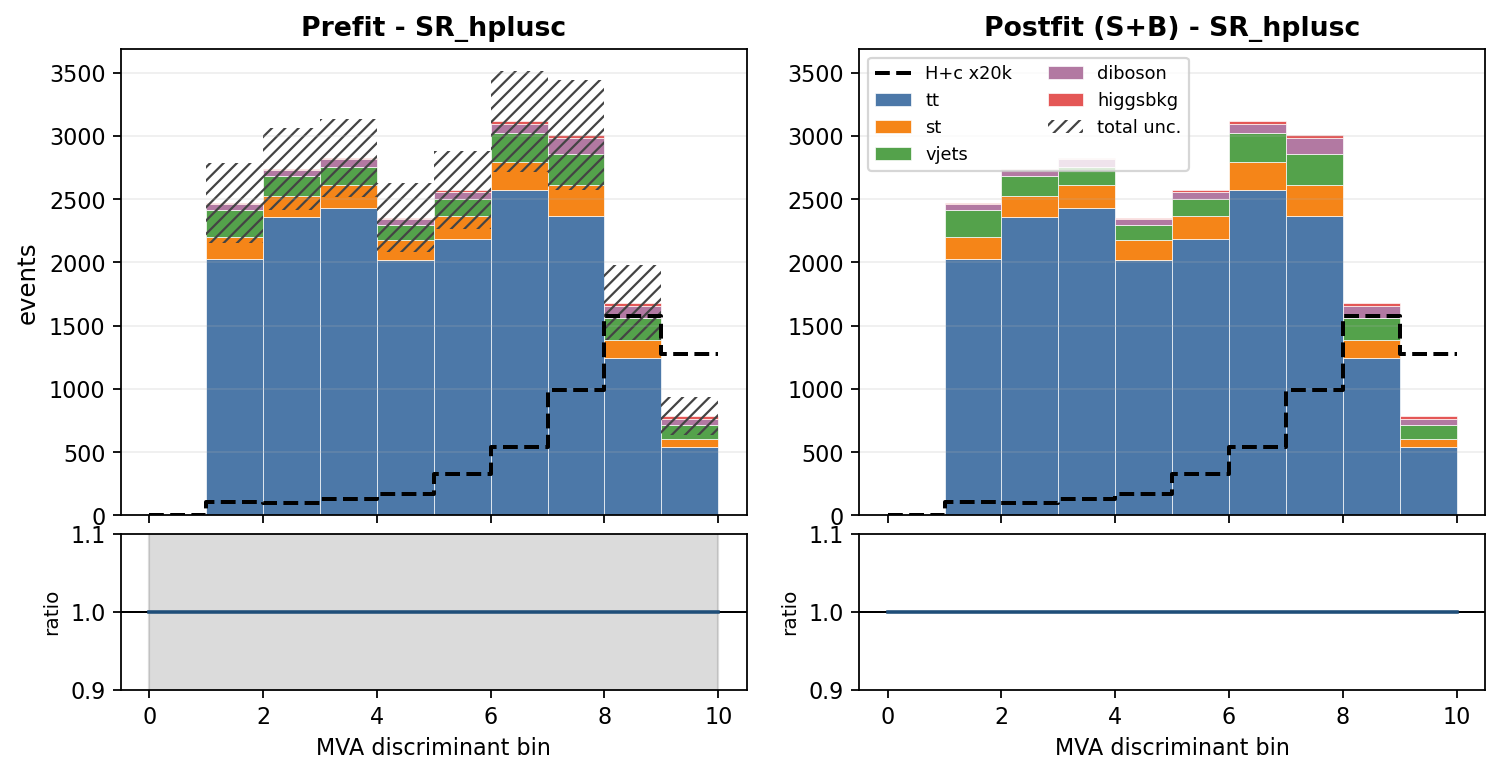
\includegraphics[width=0.80\textwidth]{img/prepost3.png}
\end{center}
\vspace{0.2em}
{\small Backgrounds stacked, H+c overlaid ($\times$20k). Hatched band =
\textbf{prefit} total uncertainty, $\approx$14\% per bin. Postfit errors are absent
because combine writes a \textbf{zero postfit covariance} on an Asimov fit.}
\end{frame}

\begin{frame}{Nuisance pulls and constraints}
\begin{center}
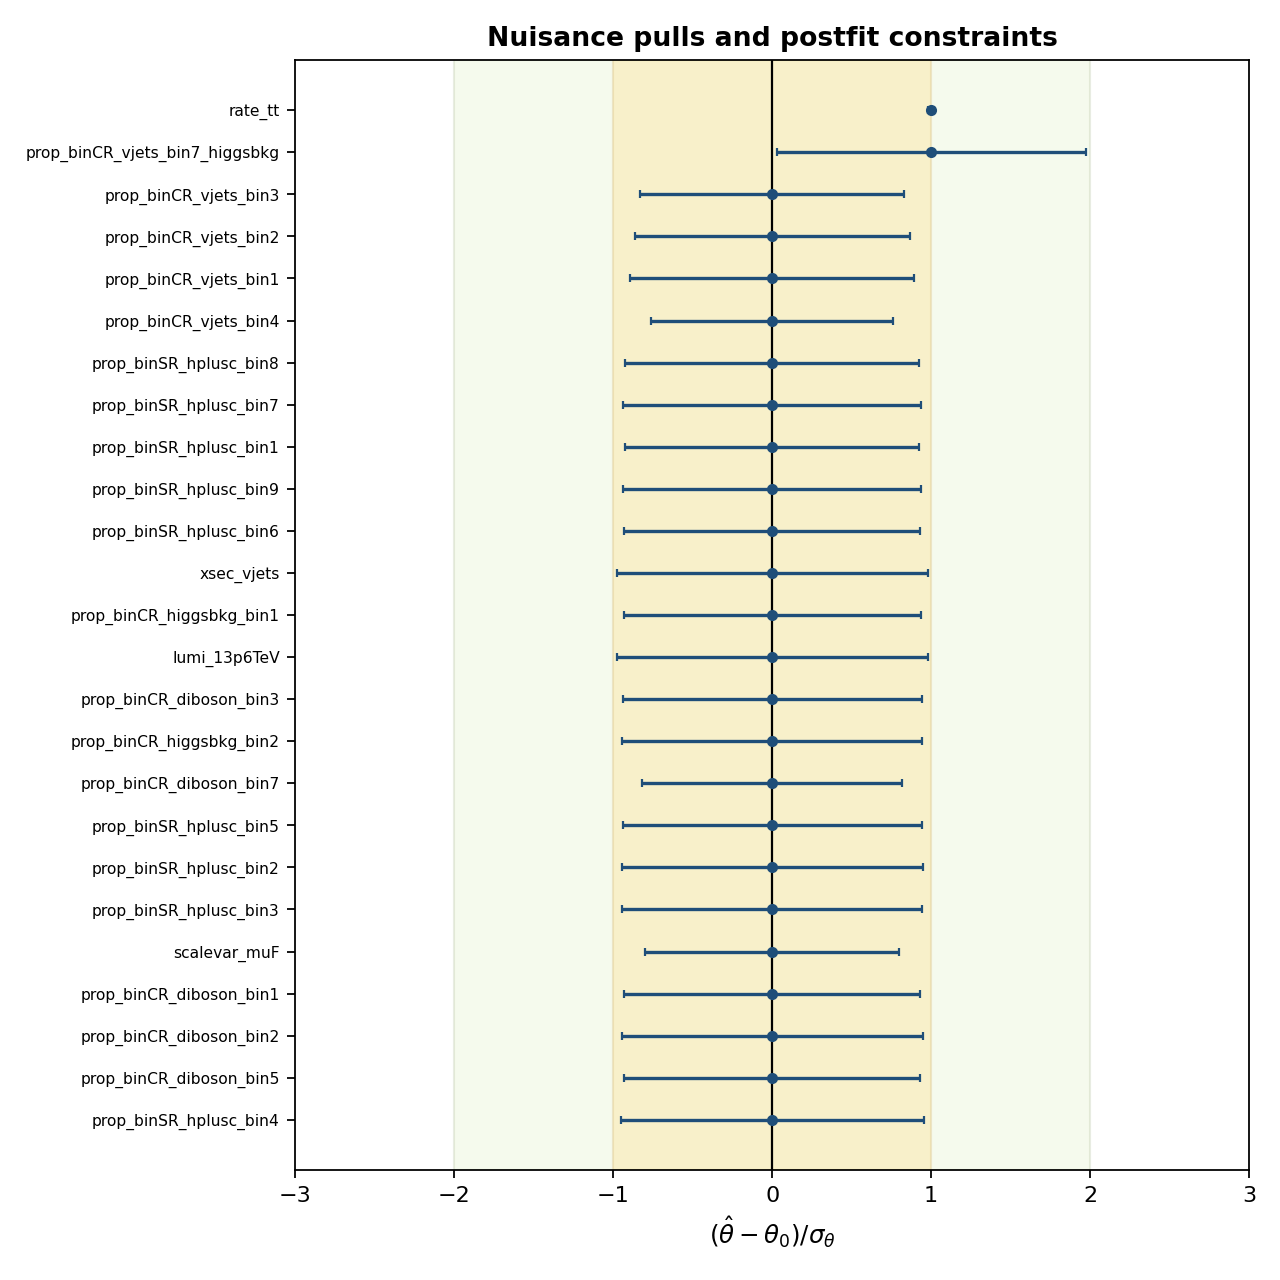
\includegraphics[height=0.76\textheight]{img/pulls.png}
\end{center}
\end{frame}

\begin{frame}{Reading the pulls}
All \textbf{Gaussian} nuisances sit at \textbf{zero pull with $\sim$unit width} ---
correct for an Asimov fit, and the check that nothing is pulled or over-constrained.
\vspace{0.3em}

The two non-zero entries are \textbf{not Gaussian} and must not be read as pulls:
\vspace{0.2em}
\begin{center}
\scriptsize
\begin{tabular}{p{0.3\textwidth}p{0.16\textwidth}p{0.44\textwidth}}
\toprule
entry & value & why \\
\midrule
\code{rate\_tt} & 1.000 $\pm$ 0.017 & free rateParam, pinned by CR\_tt \\
\code{prop\_binCR\_vjets\_bin7\_higgsbkg} & 1.000 $\pm$ 0.97 & $n_{eff}=2.1$, below
the autoMCStats threshold $\rightarrow$ an individual \textbf{Poisson} term at its
nominal scale \\
\bottomrule
\end{tabular}
\end{center}
\end{frame}

\begin{frame}{Likelihood scan}
\begin{center}
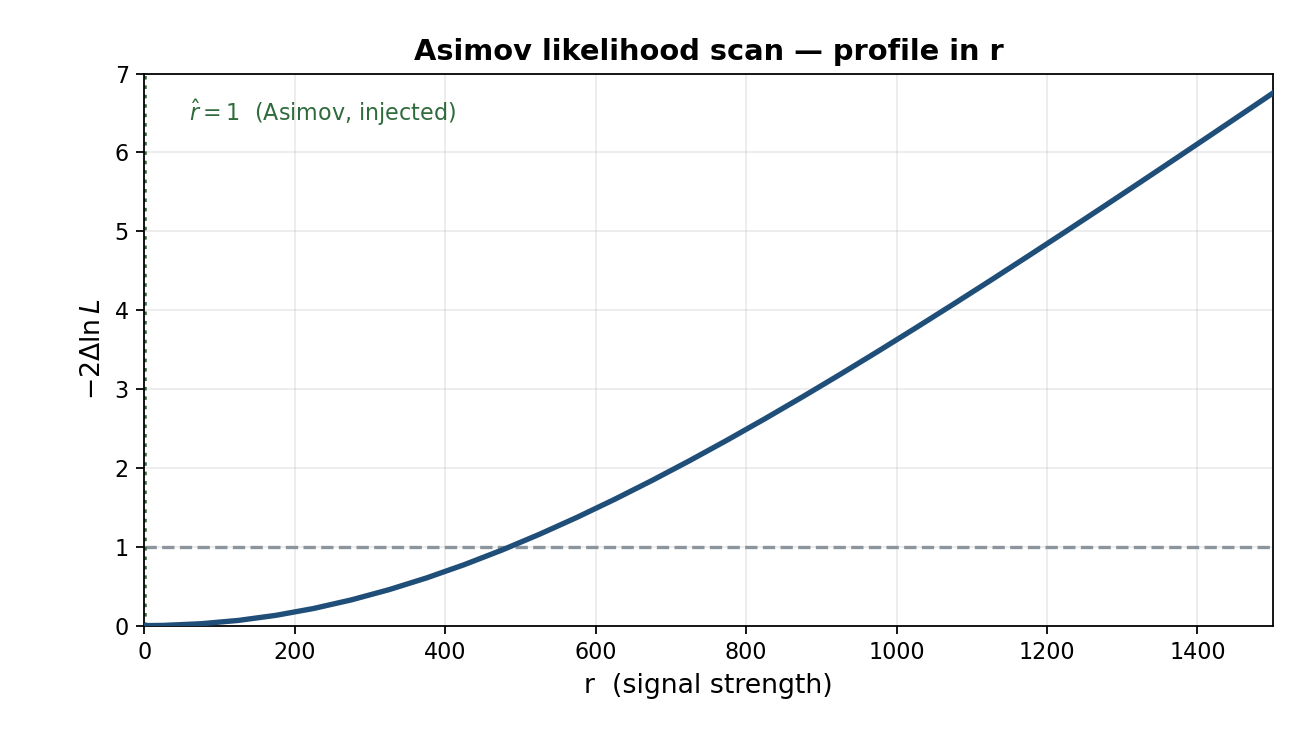
\includegraphics[width=0.62\textwidth]{img/nll_scan2.png}
\end{center}
\end{frame}

\begin{frame}{What the likelihood scan shows}
The profile likelihood in the signal strength --- all nuisances minimised at each
point in r.
\vspace{0.2em}
\begin{center}
\small
\begin{tabular}{lll}
\toprule
feature & value & meaning \\
\midrule
minimum & \textbf{$\hat{r} = 1$} & the fit recovers the injected Asimov signal --- no bias \\
$-2\Delta\ln L = 1$ & \textbf{r $\approx$ 525} & the 1$\sigma$ interval on r \\
$-2\Delta\ln L = 3.84$ & \textbf{r $\approx$ 1075} & the 2$\sigma$ crossing \\
curvature & --- & how fast the likelihood falls away = the sensitivity \\
\bottomrule
\end{tabular}
\end{center}
\vspace{0.3em}
\begin{keybox}
The 3.84 crossing (\textbf{1075}) sits close to the quoted CLs limit
(\textbf{1034}) --- the two constructions agree when the background-only and
signal+background hypotheses are well separated, which is the regime here.
\end{keybox}
\end{frame}

\begin{frame}{Nuisance impacts --- top 10}
\begin{center}
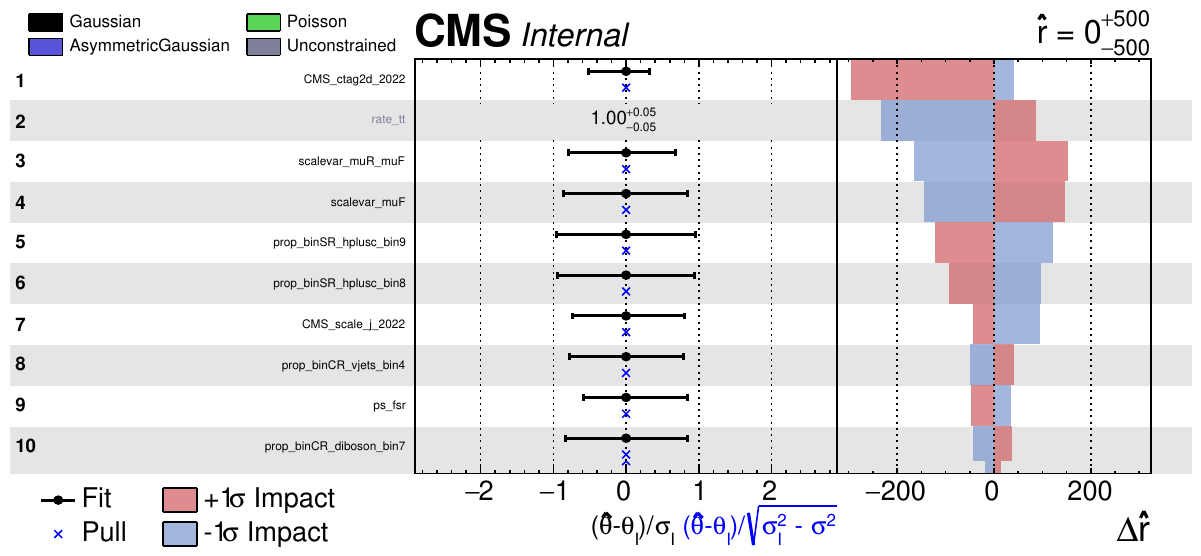
\includegraphics[width=0.84\textwidth]{img/impacts_top10.png}
\end{center}
\vspace{0.1em}
\begin{warnbox}
The header $\hat{r} = 0\ ^{+500}_{-500}$ is a \code{plotImpacts} rounding artefact
--- the actual fit returns \textbf{$\hat{r} = 0.99996$, $-513/+483$}, i.e.\ exactly
the injected Asimov value.
\end{warnbox}
\end{frame}

\begin{frame}{Reading the impacts --- the asymmetries}
{\small \textbf{Left panel} --- the pull
$(\hat\theta-\theta_0)/\sigma_\theta$. All sit at zero: this is an \textbf{Asimov}
fit, so nothing is pulled by construction.
\textbf{Right panel} --- $\Delta\hat r$ when each nuisance is moved by $\pm1\sigma$.}
\begin{keybox}
\textbf{Red (+1$\sigma$) and blue ($-1\sigma$) are not mirror images.} Three sources
of asymmetry:
\end{keybox}
\vspace{0.1em}
\begin{center}
\scriptsize
\begin{tabular}{p{0.22\textwidth}p{0.68\textwidth}}
\toprule
source & why \\
\midrule
\textbf{asymmetric lnN} & \code{xsec\_st} is \code{0.9873/1.0167} --- the up and down
variations differ by construction \\
\textbf{template shape} & up/down shifts of JES or ctag move events between bins
non-linearly \\
\textbf{re-profiling} & pushing one nuisance lets the others re-fit, and they respond
differently in each direction \\
\bottomrule
\end{tabular}
\end{center}
\vspace{0.1em}
\begin{warnbox}
The \textbf{fit range matters}: a symmetric range around $\hat r$ is required, or the
$-1\sigma$ impacts clip at the boundary and the plot comes out one-sided.
\end{warnbox}
\end{frame}

%% ===========================================================================
\sectionframe{7 \textperiodcentered\ Status and outlook}

\begin{frame}{The road so far}
\begin{center}
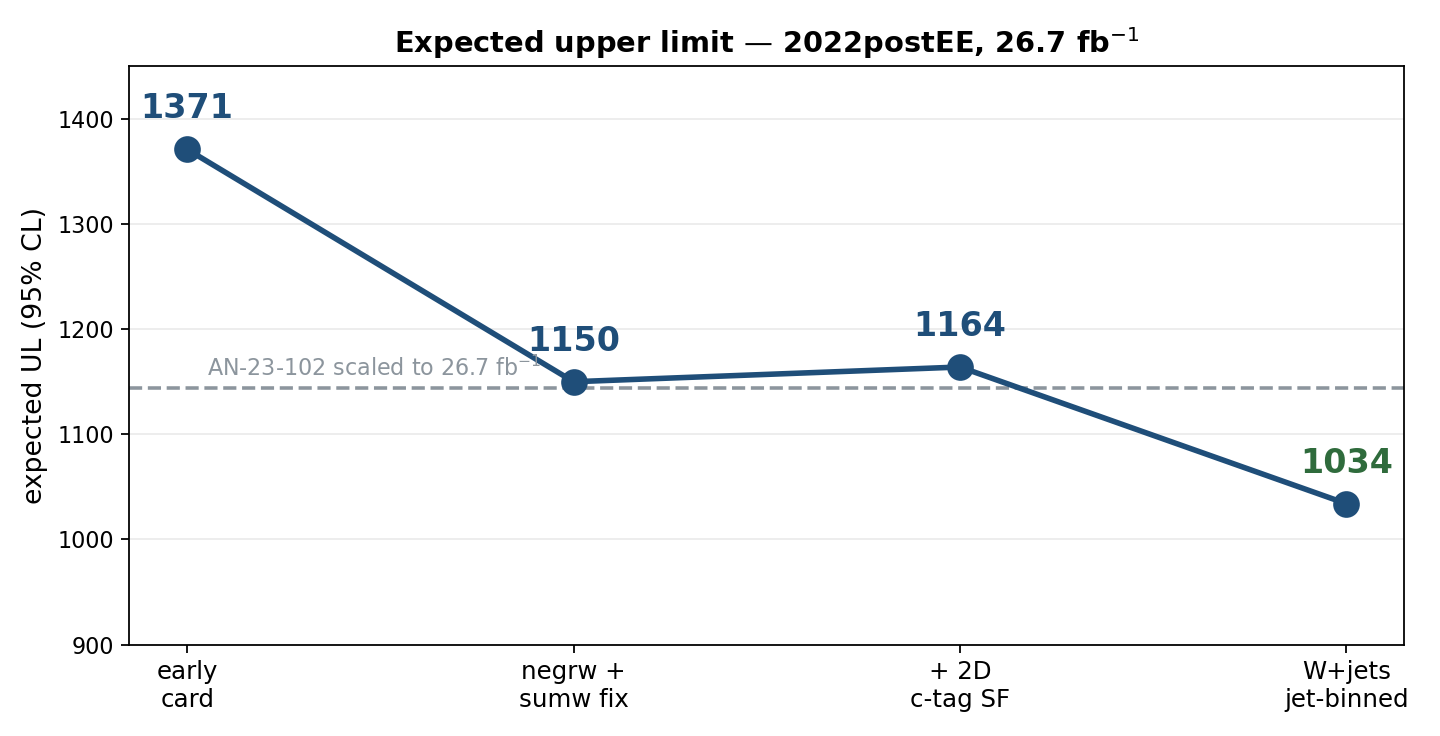
\includegraphics[width=0.82\textwidth]{img/limit_cascade.png}
\end{center}
\vspace{0.2em}
{\small Note the suppressed zero on the y-axis --- the c-tag step is a genuine but
small \textbf{+14} increase, not the spike it appears to be.}
\end{frame}

\begin{frame}{Where we stand}
\vspace{0.4em}
\begin{center}
\begin{tabular}{lr}
\toprule
 & limit \\
\midrule
AN-23-102 scaled to 26.7 fb$^{-1}$ & \textbf{1144} \\
\textbf{this analysis} & \textbf{1034} \\
our statistical only & \textbf{641} \\
\bottomrule
\end{tabular}
\end{center}
\vspace{0.4em}
\begin{keybox}
\textbf{Better than} the published analysis scaled to our luminosity --- 1034 vs
1144, a \textbf{9.6\% improvement}, on \textbf{5$\times$ less data}.
\end{keybox}
\begin{warnbox}
\textbf{The scaling is indicative.} $503\sqrt{138/26.7}=1144$ assumes a purely
statistics-limited extrapolation; the AN is 73.8\% statistical, so the true scaled
value is \textbf{worse} than 1144 --- our margin is \textbf{larger} than 9.6\%.
\end{warnbox}
\end{frame}

\begin{frame}{What is still missing}
\vspace{0.3em}
\begin{center}
\small
\begin{tabular}{ll}
\toprule
item & status \\
\midrule
\textbf{negrw retrain} & classifier to be retrained on the jet-binned W+jets samples \\
\textbf{4FS/5FS signal theory} & placeholder 1.30 --- needs re-derivation at 13.6 TeV \\
\textbf{Trigger scale factors} & implemented, \textbf{not yet enabled} \\
\textbf{Higgs heavy-flavour} (\code{higgs\_plus\_c}) & implemented, pending activation \\
\textbf{top-$p_T$ reweighting} & implemented, pending activation \\
Dataset substitutions & W+jets $p_T$-binned (full AN stitch) \\
 & DY $\rightarrow$ Z$\rightarrow\tau\tau$ filtered \\
 & tt / single-top \code{-ext} samples \\
 & \code{WZto3LNu} \\
\bottomrule
\end{tabular}
\end{center}
\end{frame}

\begin{frame}{Priorities}
\vspace{0.4em}
\begin{center}
\small
\begin{tabular}{clp{0.45\textwidth}}
\toprule
\# & item & why \\
\midrule
\textbf{1} & Re-derive \code{xsec\_hplusc\_4FS\_5FS} & 30\% flat lnN on a
statistics-starved signal \\
\textbf{2} & Enable trigger SFs & implemented, one flag \\
\textbf{3} & Activate \code{higgs\_plus\_c} + \code{top\_pt} & proper HF and tt
treatment \\
\textbf{4} & Add the missing datasets & more MC statistics \\
5 & Decorrelate \code{CMS\_ctag2d\_2022} & currently one nuisance over the whole plane \\
\bottomrule
\end{tabular}
\end{center}
\end{frame}

%% ---------------------------------------------------------------------------
{\setbeamercolor{background canvas}{bg=deckblue}
\begin{frame}[plain]
  \vfill
  \begin{center}
    {\Huge\bfseries\color{white} Summary}\\[0.6em]
    \colorbox{deckgold}{\makebox[0.3\textwidth]{\rule{0pt}{1.2pt}}}\\[1.0em]
    {\color{white} \textbf{Expected UL 1371 $\rightarrow$ 1034} \textperiodcentered\
     statistical-only \textbf{641}}\\[0.6em]
    {\color{white} V+jets $n_{eff}$ \textbf{280 $\rightarrow$ 1170}}\\[1.0em]
    {\large\color{white} Within $\sim$5\% of the Run 2 analysis scaled to our luminosity}\\[1.0em]
    {\color{white!85!deckblue}\small Remaining: 4FS/5FS re-derivation, trigger SFs,
     dataset substitutions}
  \end{center}
  \vfill
\end{frame}}

\end{document}
